\chapter{Implementation}\label{chap:imp}

\section{Overview}

The  analysis is implemented as a series of stages, firstly, the e-mail header
is parsed, to extract important information to a predefined set of Java objects.
This is followed by the analysis phase, where the resultant data is passed to a
set of analyser modules, each running separately.  Finally, this information is
presented to the user.  This chapter presents each of these stages in detail.

\subsection{Program Overview}

The program is split up into three main stages: textual analysis and parsing; header contents analysis, and visualisation, as shown in Figure~\ref{fig:con}.

\begin{figure}[!ht]
	\centering
\resizebox{0.9\textwidth}{!}{
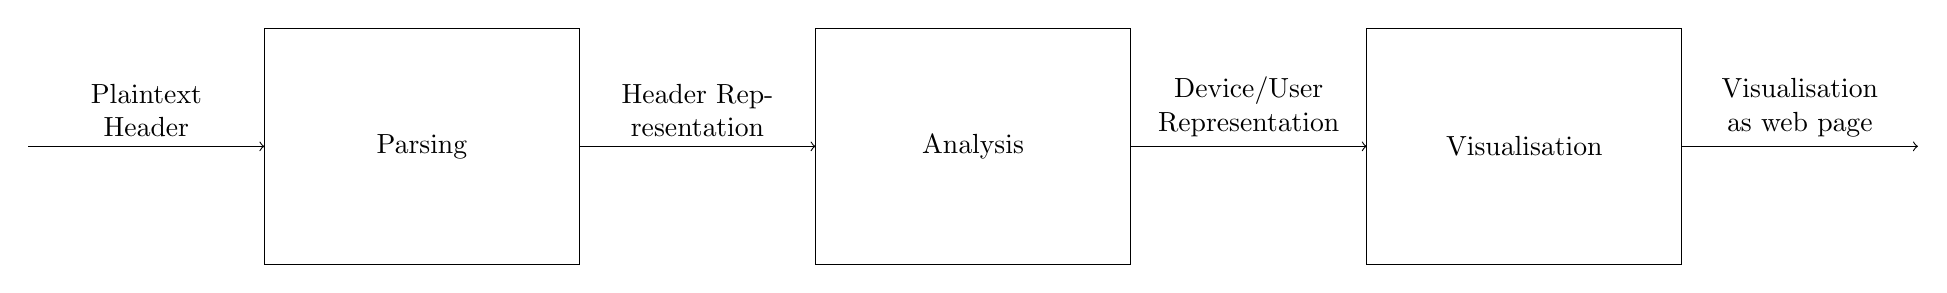
\begin{tikzpicture}
	\draw [->] (-3,1.5) -- (0,1.5) node [above, text width=2.5cm, align=center, midway] { Plaintext Header };
	\draw (0,0) rectangle node {Parsing} (4,3);
	\draw [->] (4,1.5) -- (7,1.5) node [above, text width=2.5cm, align=center, midway] { Header Representation };
	\draw (7,0) rectangle node {Analysis} (11,3);
	\draw [->] (11,1.5) -- (14,1.5) node [above, text width=2.5cm, align=center, midway] { Device/User Representation };
	\draw (14,0) rectangle node {Visualisation} (18,3);
	\draw [->] (18,1.5) -- (21,1.5) node [above, text width=2.5cm, align=center, midway] { Visualisation as web page };
\end{tikzpicture}}
\caption{Simplified Control Flow of Application}
\label{fig:con}
\end{figure}

\section{Definitions}

The following covers the essential definitions required for the notation and
concepts that will be discussed in this document.

\subsection{Parsing}

In order to aid the parsing of the e-mail header, a combination of regular
expressions and context-free grammars are needed, and defined as follows.

\paragraph{Alphabets and Languages}

A set of symbols, usually denoted as $\Sigma$.  A language is a subset of
$\mathcal P (\Sigma)$.

The following special classes are provided as part of the Perl-Compatible
Regular Expression library, and are subsets of the alphabet of Unicode
characters, defined in~\cite{php_group_gutmans_lerdorf_suraski_boerger}.

\begin{description}

\item[alnum] --- letters and digits

\item[alpha] --- letters

\item[ascii] --- the set of ASCII characters (character codes 0 --- 127)

\item[blank] --- tabs or blank spaces

\item[cntrl] --- control characters

\item[digit] --- decimal digits

\item[graph] --- printing characters (excluding spaces)

\item[lower] --- lower-case letters

\item[print] --- printing characters (including spaces)

\item[punct] --- punctuation marks (printing characters excluding letters and spaces)

\item[space] --- white space

\item[upper] --- upper case letters

\item[word] --- ``word'' characters (same

\item[xdigit] --- hexadecimal digits

\end{description}
\subsubsection{Regular Languages}
Regular languages are defined as follows:
\begin{itemize}
\item $\emptyset$ and $\{\epsilon\}$ are regular languages
\item for each $a\in\Sigma$, $\{a\}$ is a regular language
\item if $A$ and $B$ are both regular, $A\cup B$, $A\cdot B$ and $A^*$ are regular languages.
\subitem{ $A\cup B$ is the union of two languages.  $A\cup B = \{s : s\in A \lor s \in B\}$}
\subitem{ $A\cdot B$ is the concatentation of two languages.  $A\cdot B = \{ ab : a \in A, b \in B\}$}
\subitem{ $A^*$ is the Kleene star of a language.}
\begin{align*}
    A_0&=\{\epsilon\}\\
    A_1&= A\\
    A_{i+1} &= \{ aa' : a \in A_i, a'\in A\}\\
    A^* &= \bigcup_{i\in\mathbb N} A_i
\end{align*}
\end{itemize}

\subsubsection{Context-Free Grammars}
A context-free grammar $G$ is defined as $G=\left(V,\Sigma, R,S\right)$ where:
\begin{itemize}
\item $V$ is a variable.
\item $\Sigma$ is the alphabet of symbols.
\item $R$ is a relation defined over $V\rightarrow \left(V\cup\Sigma\right)^*$
\item $S$ is the start symbol
\end{itemize}

For example, $\langle \text S \rangle$ is the field name with the associated
productions $\langle \text T \rangle \, \langle \text U \rangle$, where $T$ and
$U$ are productions.

\begin{bnf*}
	\bnfprod{S}{\bnfpn{T} \bnfsp{} \bnfpn{U}}
\end{bnf*}

For example, $\langle \text S \rangle$ is the field name with the associated
productions $a \, \langle \text U \rangle$, where $a$ is a terminal symbol.

\begin{bnf*}
	\bnfprod{S}{\bnftd{a} \bnfsp{} \bnfpn{U}}
\end{bnf*}
This is then extended in the following ways used in the RFC syntax.

The square brackets are used to indicate an optional element.
\begin{bnf*}
\bnfprod{field}{\bnfpn{field-name} \bnfts{:} \bnfsp{}[ \bnfpn{field-body} ]\bnfsp{} \bnfts{CRLF}}\\
\end{bnf*}

The asterisk is used to indicate an element that appears 0 or more times. $n*$
is used to indicate a component that repeats $n$ or more times.

\begin{bnf*}
\bnfprod{fields}{\bnfpn{dates}\bnfsp \bnfpn{source} \bnfsp 1\!*\bnfpn{destination} \bnfsp * \bnfpn{optional-fields}}\\
\end{bnf*}

The hash-symbol is used to indicate an element that appears a certain number of
times. $m*n$ is used to indicate a component that repeats at least $m$ times and
at most $n$ times.

\begin{bnf*}
\bnfprod{fields}{\bnfpn{dates}\bnfsp \bnfpn{source} \bnfsp 1\!\#\bnfpn{destination} \bnfsp * \bnfpn{optional-fields}}\\
\end{bnf*}

The $|$ is used to indicate a selection between a pair of elements.
\begin{bnf*}
\bnfprod{fields}{\bnfts{a}\bnfor \bnfts{b}}\\
\end{bnf*}

\subsection{Database Queries}
The following notations will be used for the CVE database queries.

\paragraph{Set-Theoretic Operators}
The operators $F\cup G$, $F \cap G$, $F\setminus G$ behave as is expected for
these operators, resulting in the union, intersection and difference of the
sets.  The only proviso being that the atrribute names must match.

\paragraph{Selection} \[\sigma_{\text{product}=\text{thunderbird}}D\]
The above notation is used to indicate a search over the attribute named
``product'' for the string ``thunderbird'' in the database table $D$.  As a
single database is only being used, this may be occasionally elided.  The output
of this function is another object of the same type as $D$.

\paragraph{Projection}
\[\pi_{\text{product}}D\]
The above notation is used to indicate a projection on the attribute named
``product'' in the database table $D$.  The output of this function is another
object of the same type as $D$.

\paragraph{Composition}
The above functions results can be coposed repeatedly to produce more specific
search queries.

\subsection{Data Structures}
These wil be drawn using square boxes to represent single objets that are encapsulated
within an object.  Square boxes with an inner square box indicate some collection
of objects.

Thin arrows will be used to denote the encapsulation relation, with thicker
arrows being used to list relevant public methods.

\section{Data Extraction and Parsing}

The parser's operation completes in a number of stages, following RFC822
(\cite{RFC0822}).  The header is divided up into two disjoint sections, the
routing information (\texttt{Received from...}) and the key-value map of other
pertinent information.

\subsection{Received fields}

The received fields are the most complicated part of the e-mail header to parse,
as they are described by a non-trivial grammar, presented below.

\begin{bnf*}
\bnfprod{message}{\bnfpn{fields}\bnfsp *(\bnfts{CRLF} \bnfsp *\bnftd{text})}\\
\bnfprod{fields}{\bnfpn{dates}\bnfsp \bnfpn{source} \bnfsp 1\!*\bnfpn{destination} \bnfsp * \bnfpn{optional-fields}}\\
\bnfprod{field}{\bnfpn{field-name} \bnfts{:} \bnfsp [ \bnfpn{field-body} ]\bnfsp \bnfts{CRLF}}\\
\bnfprod{field-name}{\bnftd{any word consisting of CHAR, excluding CTLs, SPACE, and ``'':''}} \\
\bnfprod{field-body}{\bnfpn{field-body-contents} \bnfsp [\bnfts{CRLF} \bnfsp \bnftd{LWSP-char}\bnfsp  \bnfpn{field-body}]}\\
\bnfprod{field-body-contents}{\bnftd{ASCII characters}}\\
\bnfprod{source}{[\bnfpn{trace}] \bnfsp \bnfpn{originator} [\bnfpn{resent}]}\\
\bnfprod{trace}{\bnfpn{return}\bnfsp 1\!* \bnfpn{received}}\\
\bnfprod{return}{\bnfts{Return-path:}\bnfsp{} \bnfpn{route-addr}}\\
\bnfprod{recieved}{\bnfts{Received:}}\\
\bnfprod{cont.}{[\bnfts{from}\bnfsp\bnfpn{domain}]}\\
\bnfprod{cont.}{[\bnfts{by}\bnfsp\bnfpn{domain}]}\\
\bnfprod{cont.}{[\bnfts{via}\bnfsp\bnfpn{atom}]}\\
\bnfprod{cont.}{*(\bnfts{with}\bnfsp\bnfpn{atom})}\\
\bnfprod{cont.}{[\bnfts{id}\bnfsp\bnfpn{msg-id}]}\\
\bnfprod{cont.}{[\bnfts{for}\bnfsp\bnfpn{addr-spec}]}\\
\bnfprod{cont.}{\bnfts{;}\bnfsp\bnfpn{date-time}}\\
\bnfprod{msg-id}{\bnfts{$<$}\bnfpn{addr-spec}\bnfts{$>$}}\\
\bnfprod{addr-spec}{\bnfpn{local-part}\bnfsp\bnfts{@}\bnfsp\bnfpn{domain}}\\
\bnfprod{local-part}{\bnfpn{word}\bnfsp *(\bnfts{.}\bnfsp\bnfpn{word})}\\
\bnfprod{word}{\bnfpn{atom}\bnfor\bnfpn{quoted-string}}\\
\bnfprod{domain}{\bnfpn{sub-domain} *(\bnfts{.}\bnfpn{sub-domain})}\\
\bnfprod{sub-domain}{\bnfpn{domain-ref}\bnfor\bnfpn{domain-literal}}\\
\bnfprod{domain-ref}{\bnfpn{atom}}\\
\bnfprod{date-time}{[ \bnftd{day,} ] \bnfsp \bnftd{date}\bnfsp \bnftd{time}}\\
\bnfprod{atom}{1\!*\bnftd{any character excluding specials, SPACE and CTLs}}\\
\end{bnf*}

An example field is as follows:
\begin{verbatim}
Received: from relay12.mail.ox.ac.uk (129.67.1.163)
    by HUB05.ad.oak.ox.ac.uk (163.1.154.231)
    with Microsoft SMTP Server id 14.3.169.1;
    Sat, 14 Nov 2015 10:55:35 +0000
\end{verbatim}
\subsection{Other fields}

These are read by a Python script and output to \texttt{STDOUT} to be read by
the Java parser in a consistent format.  These are then loaded into a hashmap to
allow quick lookup.

\section{Analysis}

After completing the parsing of the fields, it is then ready to be analysed for
different features.  All of the analysers implement the \texttt{HeaderAnalyser}
interface, requiring information about the header to be analysed, and the
currently running application.  All of these then implement the
\texttt{Runnable} interface, allowing the class to be run asynchronously.

\subsection{Input Data Structures}
The data structure presented in Figure~\ref{fig:hea} shows the output of the
parsing and textual analysis module, which is then provided as an input to the
analysis modules.

\begin{figure}[!ht]
\centering
\resizebox{0.9\textwidth}{!}{
	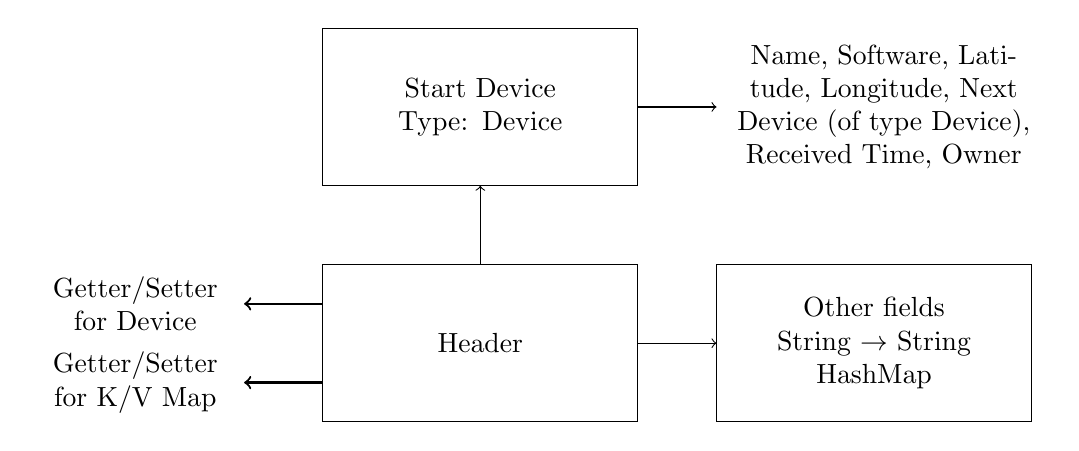
\begin{tikzpicture}
		\draw (0,0) rectangle node {Header} (4,2);
		\draw (0,3) rectangle node [text width = 3.5cm, align=center] {Start Device\\Type: Device} (4,5);
		\draw (5,0) rectangle node [text width = 3.5cm, align=center]
		{Other fields\\String $\rightarrow$ String HashMap} (9,2);
		\draw [->] (2,2) -- (2,3);
		\draw [->] (4,1) -- (5,1);
		\draw [->] (4,4) -- (5,4) node [right, text width = 4cm,align=center] { Name, Software, Latitude, Longitude, Next Device (of type Device), Received Time, Owner};
		\draw [->,thick] (0,1.5) -- (-1,1.5) node [left, text width = 2.5cm,align=center] { Getter/Setter for Device};
		\draw [->,thick] (0,0.5) -- (-1,0.5) node [left, text width = 2.5cm, align=center] { Getter/Setter for K/V Map};
\end{tikzpicture}
	}
	\caption{Header Data Structure Format}
	\label{fig:hea}
\end{figure}

\subsection{Text-Based}

The fields from the header are analysed in different modules, with searches
being performed for specific strings.  Of particular interest to Oxford Nexus
users is the ``X-Oxford-Username'' string, containing the username of the
individual that sent the message.  As confirming the username is a fairly
standard security procedure for an IT support technician, having access to this
information could allow a phisher in a later stage of an attack to increase
their credibility.

In some cases, the likely keys that are being searched for are known in advance,
and can then be checked against the hash-map of entries.

An example of this approach is for the specific check for an Oxford username, as shown in Algorithm~\ref{alg:oxf}.

\begin{algorithm}[!ht]
	\KwIn{Header}
	\KwOut{Any Oxford-based username that is found}
	\If{\texttt{X-Oxford-Username} $\in$ Header.KvMap}{ \Return{Header.KvMap(X-Oxford-Username)}\; }
	\caption{Lookup based on a known key}
	\label{alg:oxf}
\end{algorithm}

Alternatively, we may be interested in properties of the keys, necessitating a search over the keys, as shown in Algorithm~\ref{alg:exc}.

\begin{algorithm}[!ht]
	\KwIn{Header}
	\KwOut{Any information relating to Microsoft Exchange that is found}
	\ForEach{Key $k\in $ Header.KvMap}{
		\If{$k$ starts-with \texttt{X-MS-Exchange}}{
			\Return{Header.KvMap($k$)}\;
		}
	}
	\caption{Lookup based on a key property}
	\label{alg:exc}
\end{algorithm}

\subsection{Client Inferrence}

In \cite{nurse2015investigating}, a number of different e-mail clients were identified based on the header tags that were present. By identifiying these pieces of software likely to be found on a user's machine, we gain a significant amount of information from them, and should therefore devote some effort to correctly identifying them.  Using a number of e-mail samples provided, I have been able to extract examples for a number of different e-mail clients, and use them to infer the client being used.  Using a sample of e-mails, it is possible to find information for additional e-mail clients and senders, such as (but not limited to) PHPMailer and Foxmail.  A number of these approaches are shown in Algorithm~\ref{alg:inf}.

\begin{algorithm}[!ht]
	\KwIn{Header}
	\KwOut{The name of the software that is likely being used, and necessary CVE Product name (elided for brevity)}
	\uIf{``Message-ID''${}\in{}$Header.KvMap}{
		\If{Header.KvMap(``Message-ID'') contains ``email.android.com''}{
			\Return{``Android Device''}\;
		}
	}
	\uElseIf{``X-Mailer''${}\in{}$Header.KvMap}{
		\Switch{Header.KvMap(``X-Mailer'') contains}{
			\Case{``iPhone''}{\Return{``iPhone''}}
			\Case{``Outlook Express''}{\Return{``Microsoft Outlook Express''}}
			\ldots
		}
	}
	\uElseIf{``User-Agent''${}\in{}$Header.KvMap}{
		\Return{``Thunderbird''}\;

	}
	\ElseIf{Header.KvMap${}\cap{}$OutlookKeywords${}\neq\emptyset$}{
		\eIf{``X-Mailer''${}\in{}$Header.KvMap}{ \Return{Apple Mail}}{ \Return{Outlook}}

	}
	\caption{Client Inferrence Technique}
	\label{alg:inf}
\end{algorithm}


\subsection{Database Queries}

Using the results gathered from the text-based queries and analysis of the
received fields, relevant software configurations are extracted and queried
against results in the CVE database.  These are then parsed and collated in
preparation for displaying the outputs. Specifically, the queries are limited
to those matching the product name, and vulnerabilities that can be remotely
executed.

As more information is found, more details of products used will also become
available.  These are added asynchronously.

\begin{algorithm}[!ht]
	\KwIn{Header product name $p$}
	\KwOut{CVE Entries}
	cve-list $\gets\emptyset$\;
	\ForEach{$s\in\sigma_{\text{vector}\neq\text{LOCAL}}\sigma_{\text{product}=p} D$}{
		cve-builder$\gets$blank cve\;
		cve-builder.id$\gets\pi_{\text{CVE-ID}} s$\;
		$\ldots$ -- extract other features\;
		cve-list $\gets$ cve-list${}\cup{}$make(cve-builder)\;
	}
	\Return{cve-list}\;
	\caption{Extracting CVE entries}
\end{algorithm}

\section{Visualising the Results}

Using a pre-existing template, the results from the e-mail analysis will be
presented in a temporary webpage, which can then be saved independently.  Other
than the referenced JavaScript libraries, the document requires no additional
information or database access, allowing it to be quickly shared.
